\section{Limb Error Estimation}
\label{sec:limb_error_estimation}

The results for the limb error estimation are the same as for the full body error estimation. The model is overfitting and therefore only predicts the error label $0$ - No Error for most cases. The results of the training process of the Limb model can be seen in Figure \ref{fig:limb_training_results}.


\begin{figure}
  \centering
  \begin{subfigure}[b]{0.9\linewidth}
      \centering
      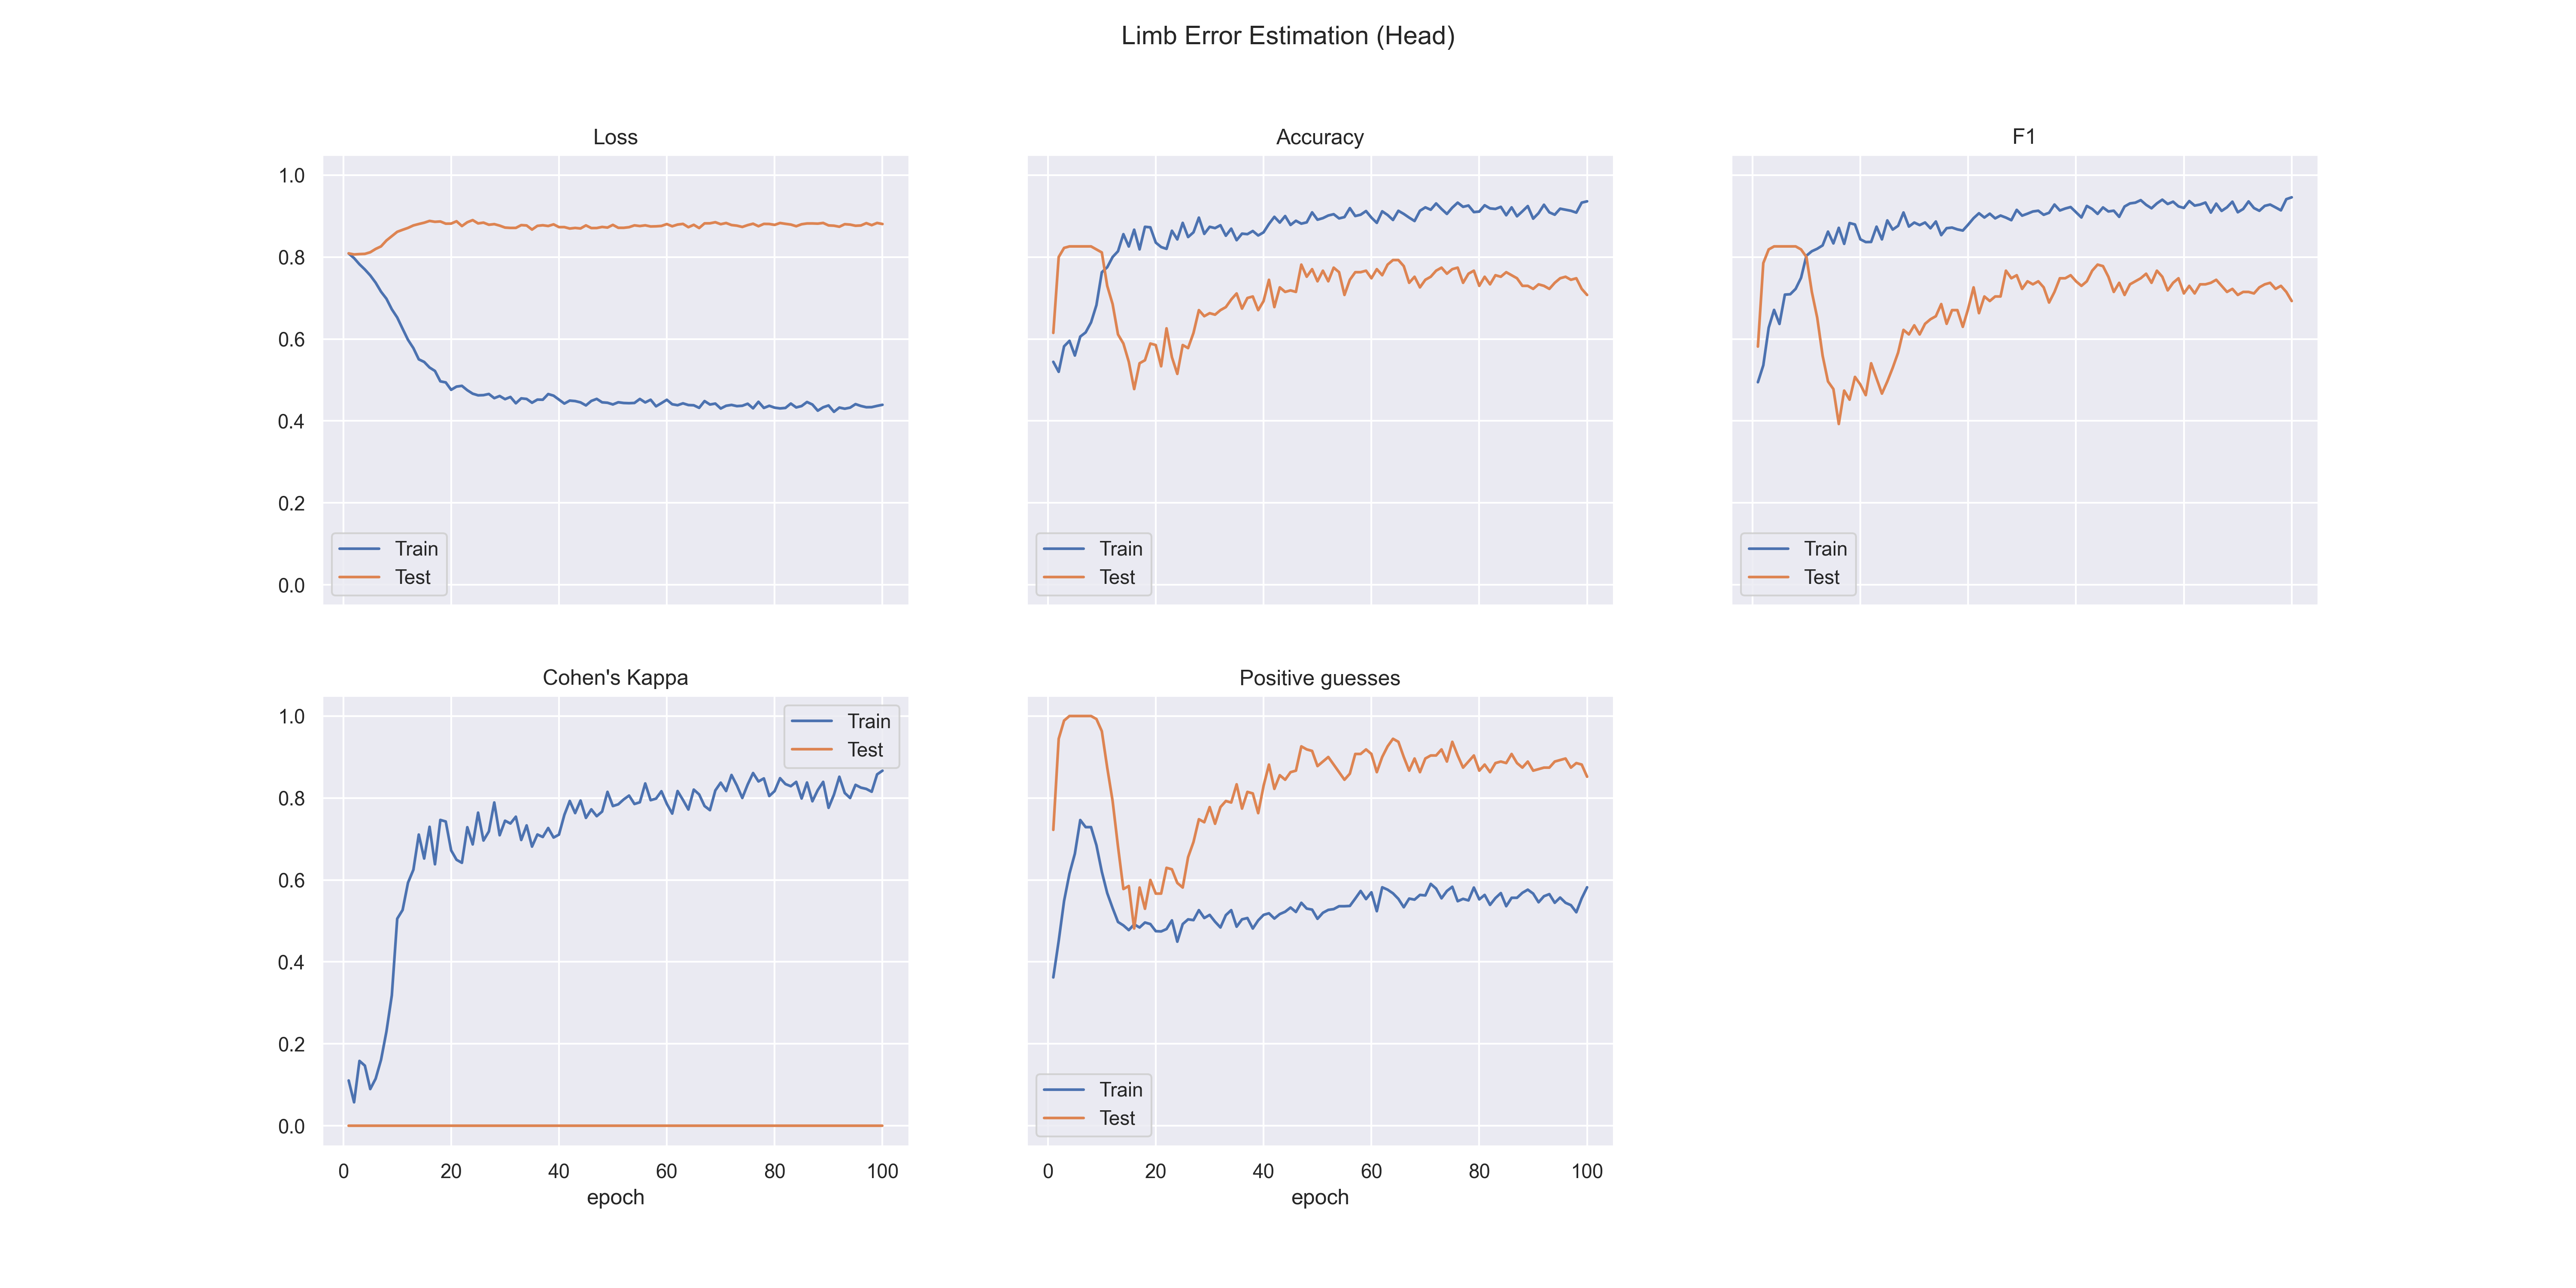
\includegraphics[width=\textwidth]{figures/Results/lb/LimbErrorEstimation_Head.png}
      \caption{Head Error Estimation}
      \label{fig:head_lb_ee}
  \end{subfigure}
  \hfill
  \begin{subfigure}[b]{0.9\linewidth}
      \centering
      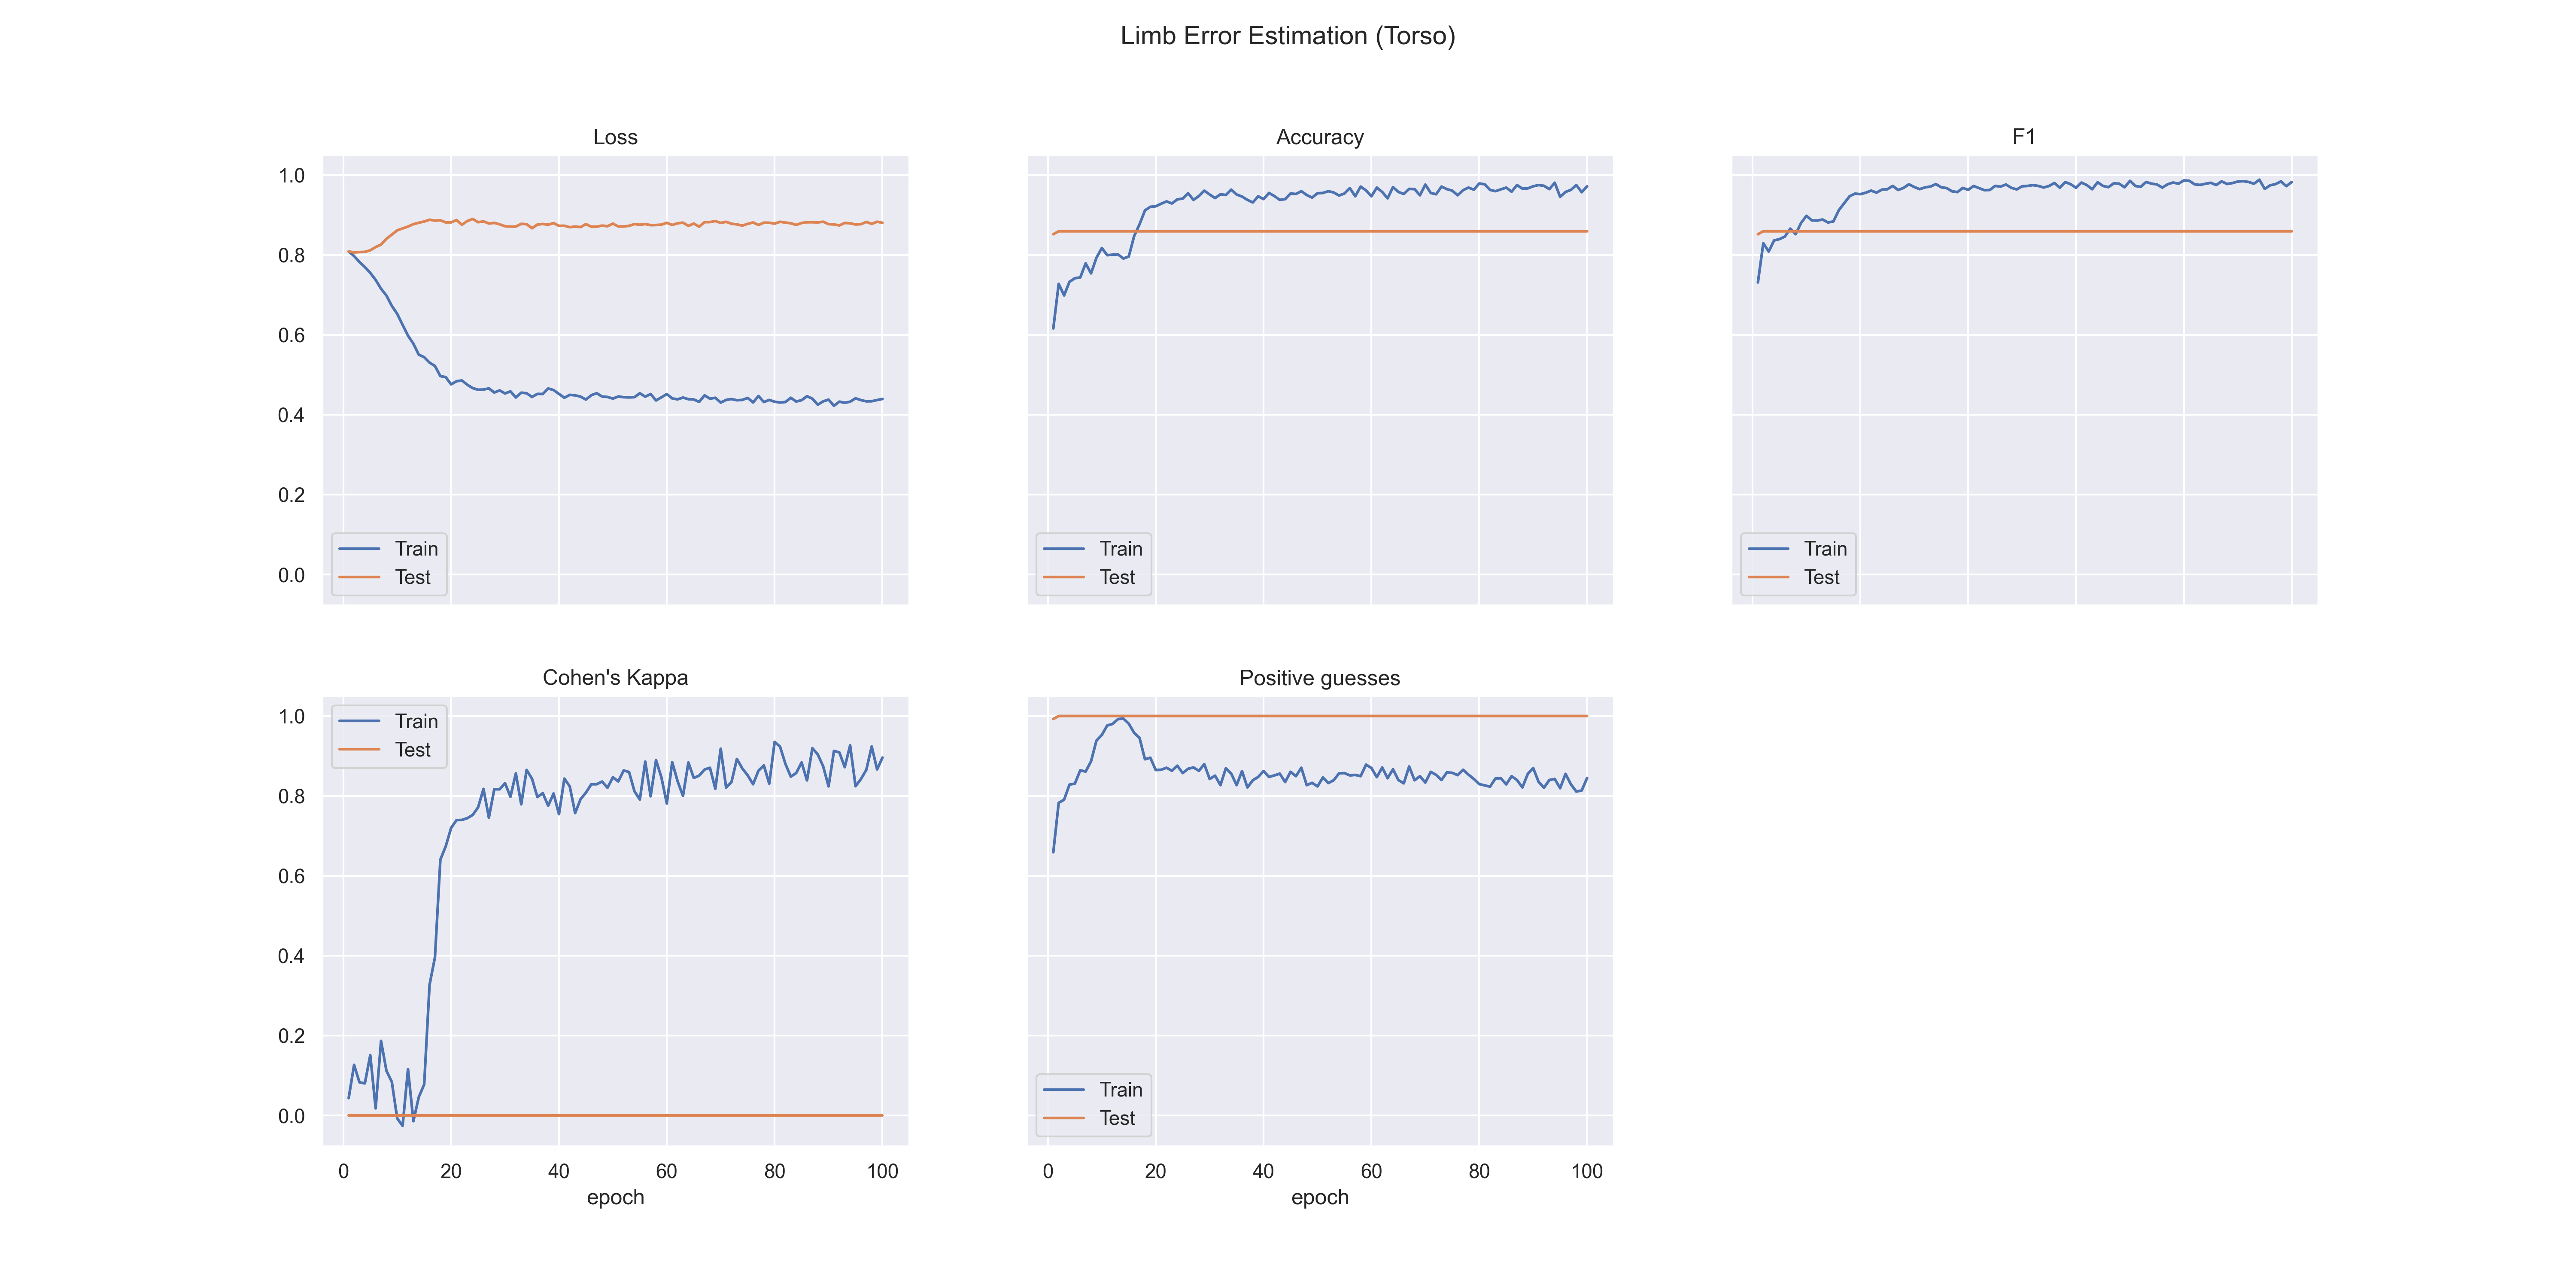
\includegraphics[width=\textwidth]{figures/Results/lb/LimbErrorEstimation_Torso.png}
      \caption{Head Error Estimation}
      \label{fig:torso_lb_ee}
  \end{subfigure}
  \hfill
  \begin{subfigure}[b]{0.9\linewidth}
      \centering
      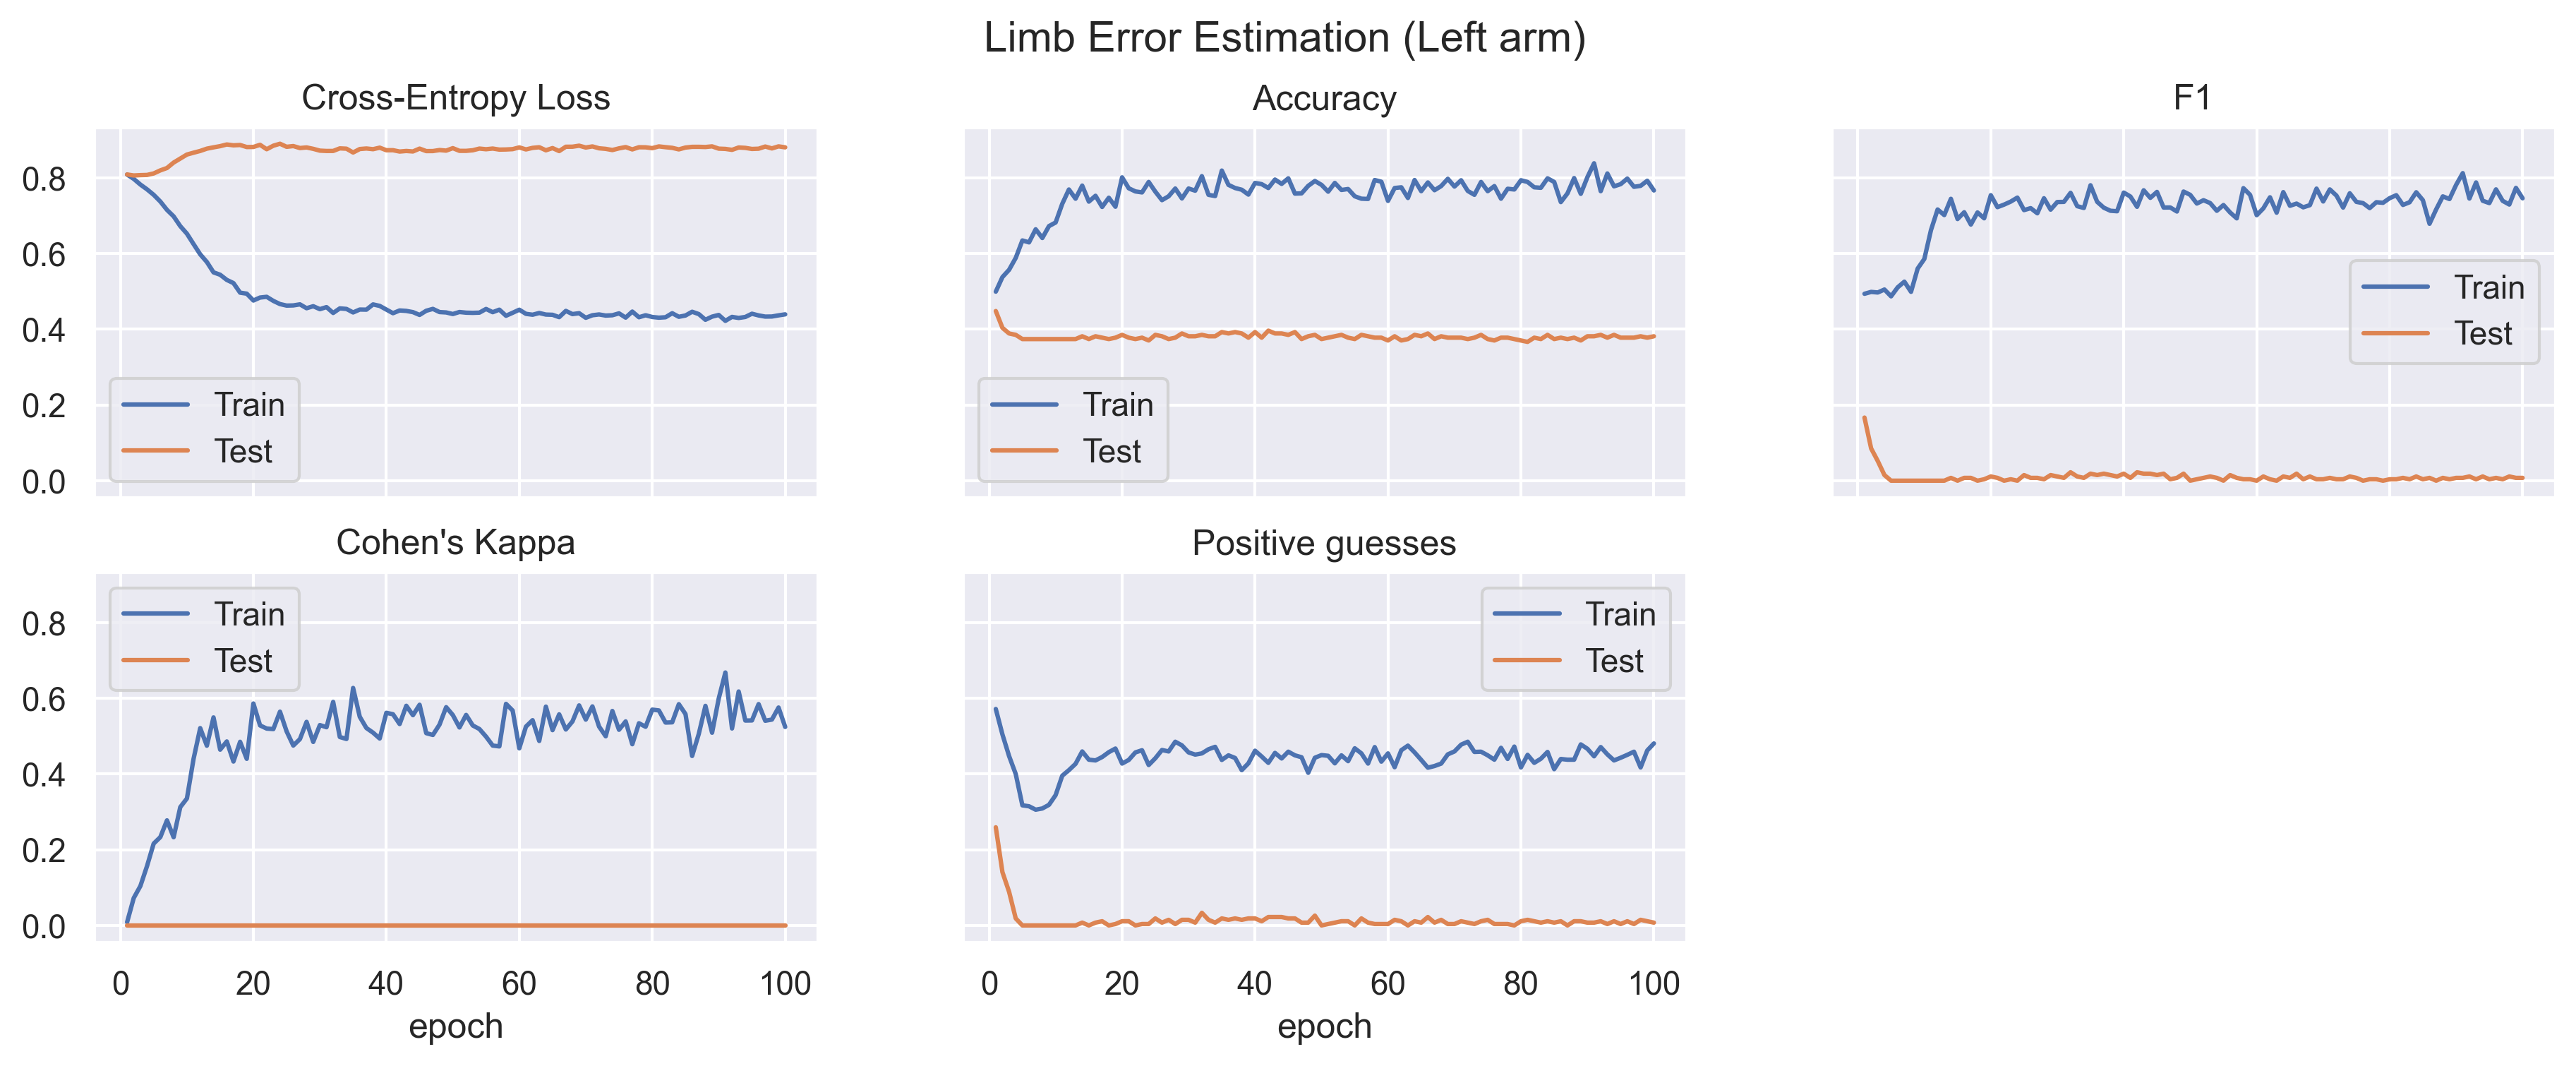
\includegraphics[width=\textwidth]{figures/Results/lb/LimbErrorEstimation_Left arm.png}
      \caption{Left Arm Error Estimation}
      \label{fig:lear_lb_ee}
  \end{subfigure}
\end{figure}

\begin{figure}
  \begin{subfigure}[b]{0.9\linewidth}
      \centering
      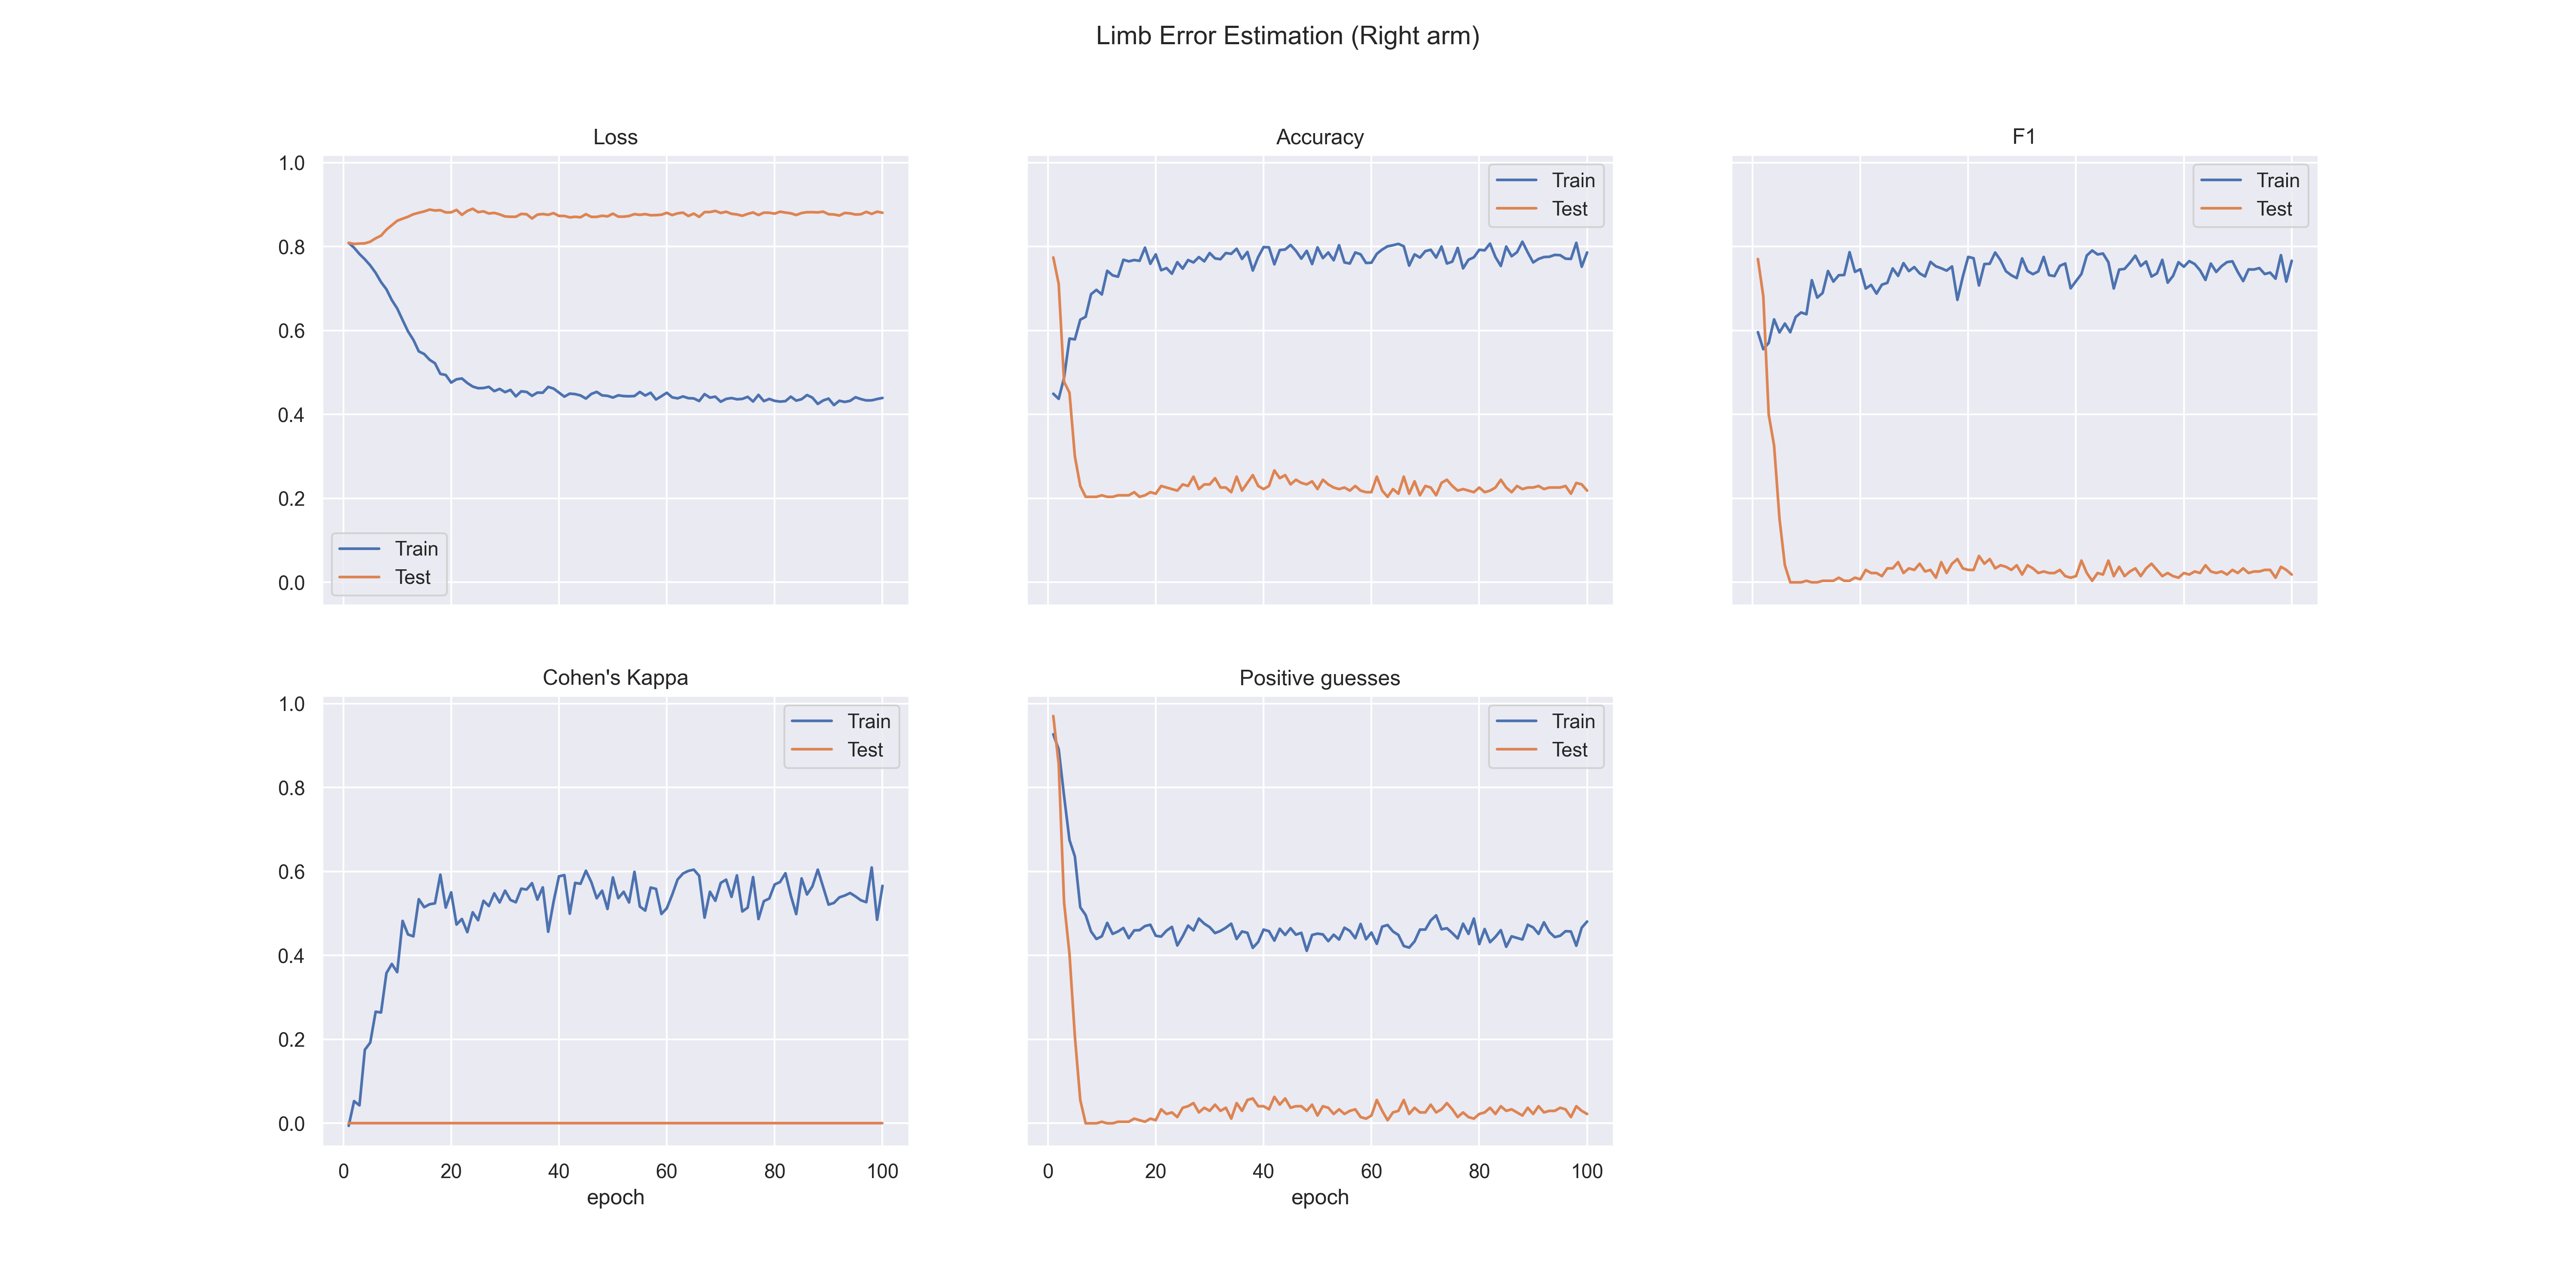
\includegraphics[width=\textwidth]{figures/Results/lb/LimbErrorEstimation_Right arm.png}
      \caption{Right Arm Error Estimation}
      \label{fig:riar_lb_ee}
  \end{subfigure}
  \hfill
  \begin{subfigure}[b]{0.9\linewidth}
      \centering
      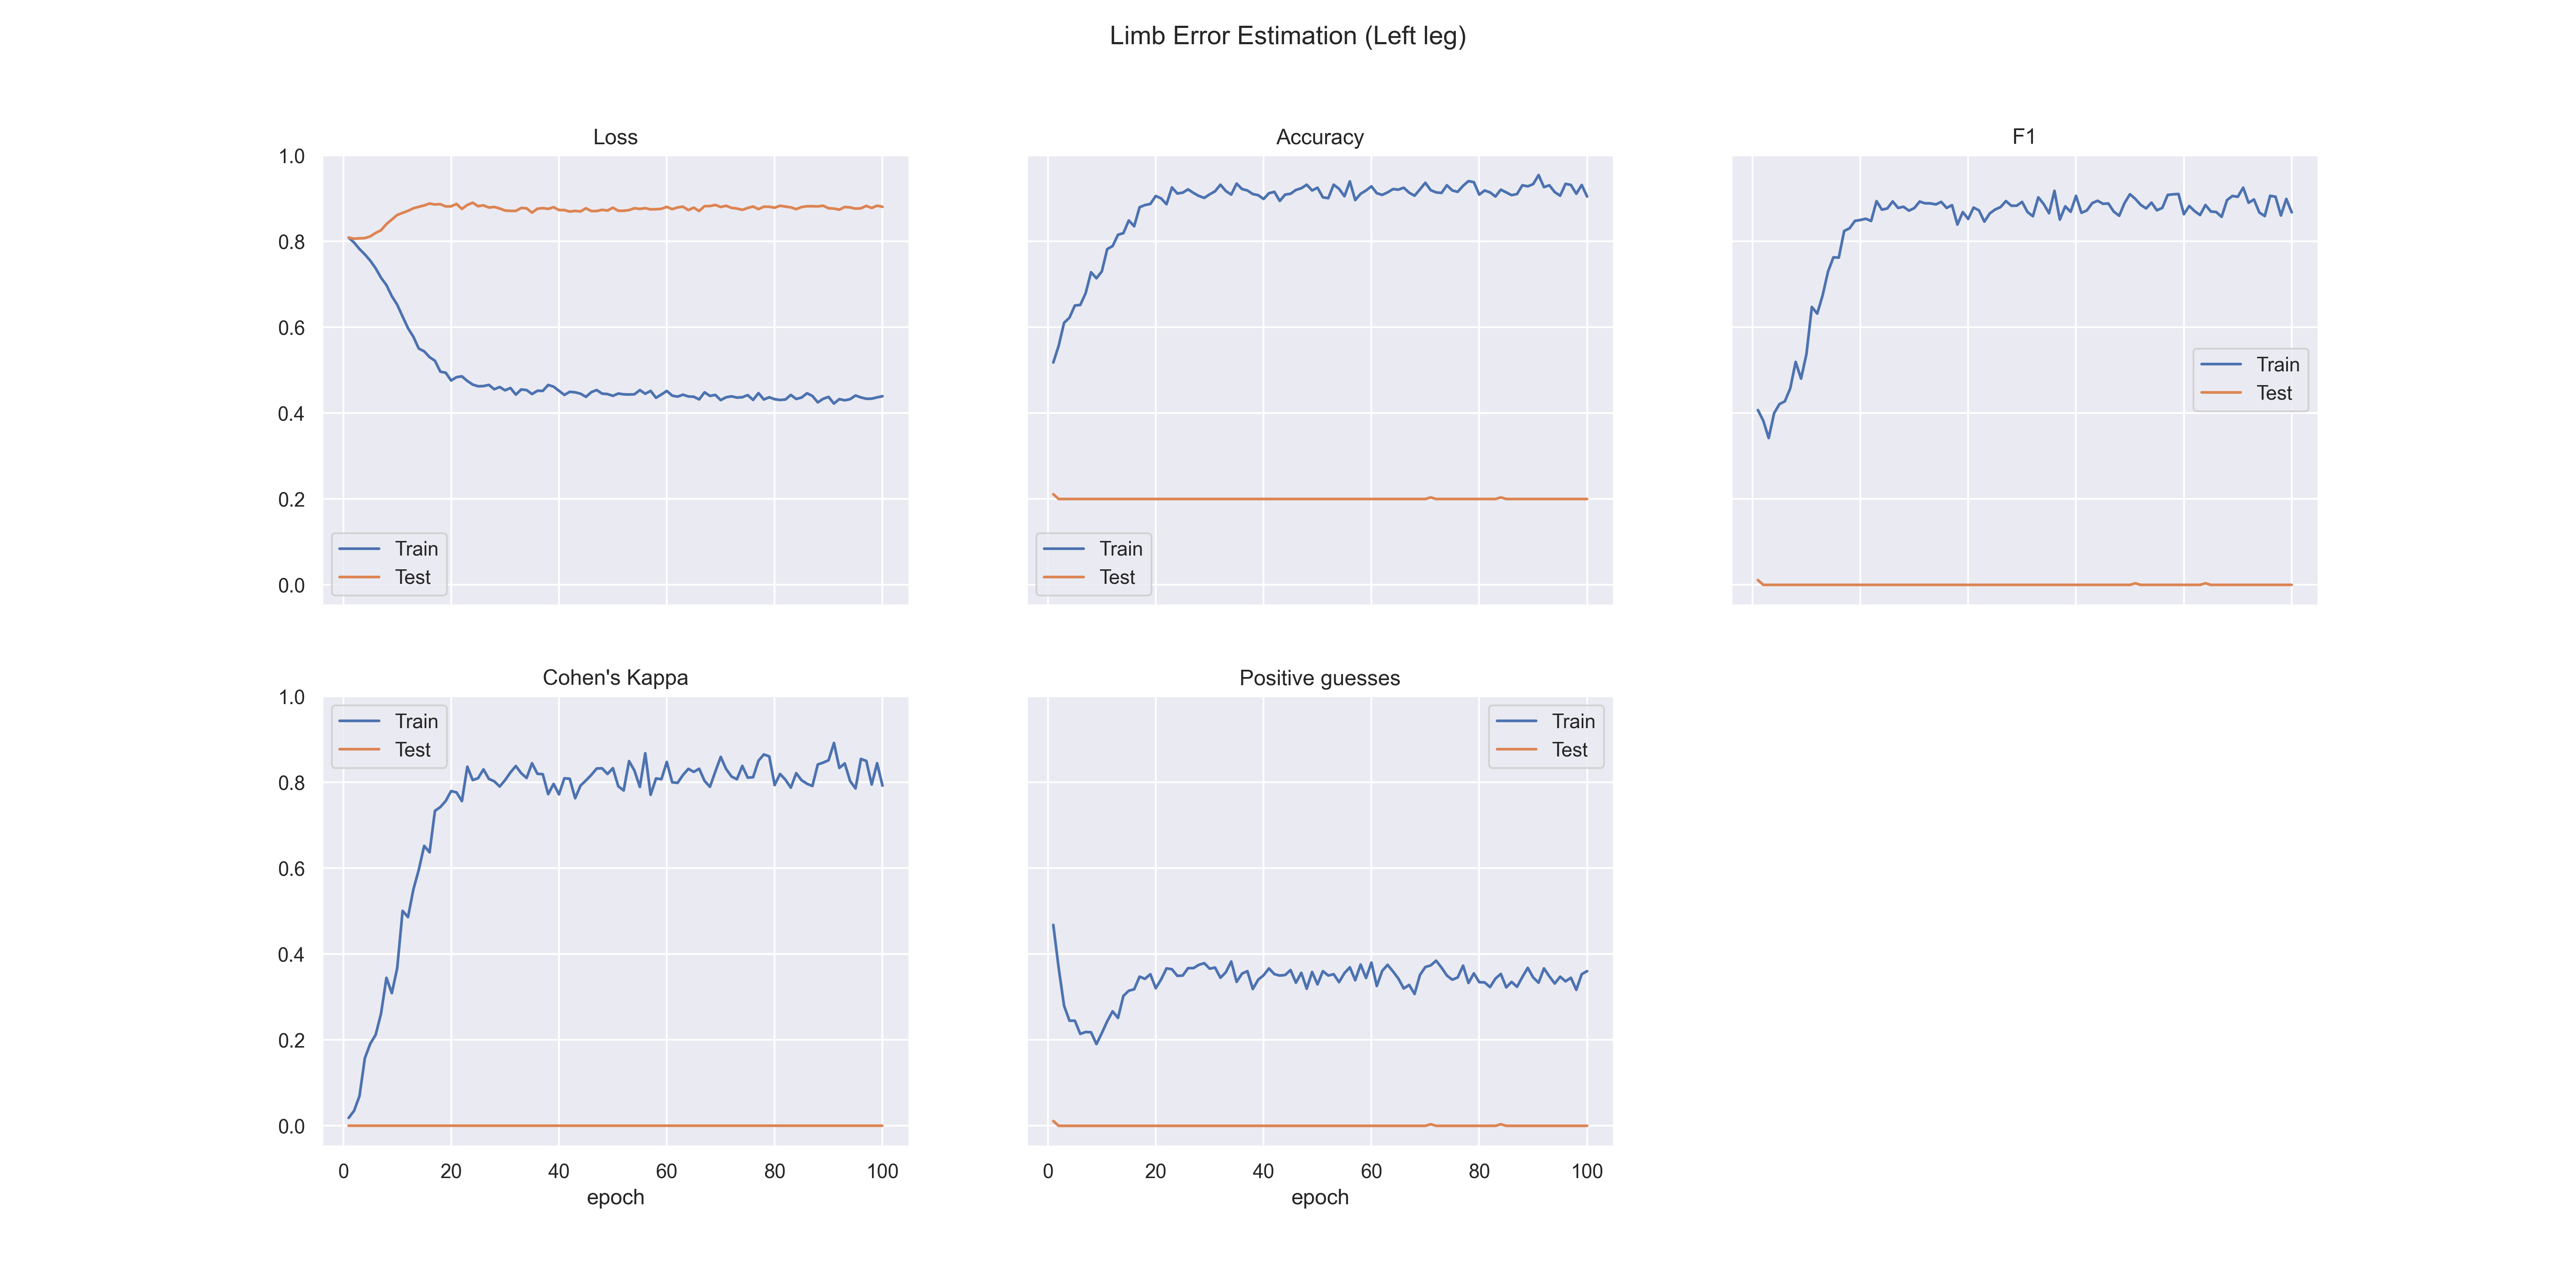
\includegraphics[width=\textwidth]{figures/Results/lb/LimbErrorEstimation_Left leg.png}
      \caption{Left leg Error Estimation}
      \label{fig:lele_lb_ee}
  \end{subfigure}
  \hfill
  \begin{subfigure}[b]{0.9\linewidth}
      \centering
      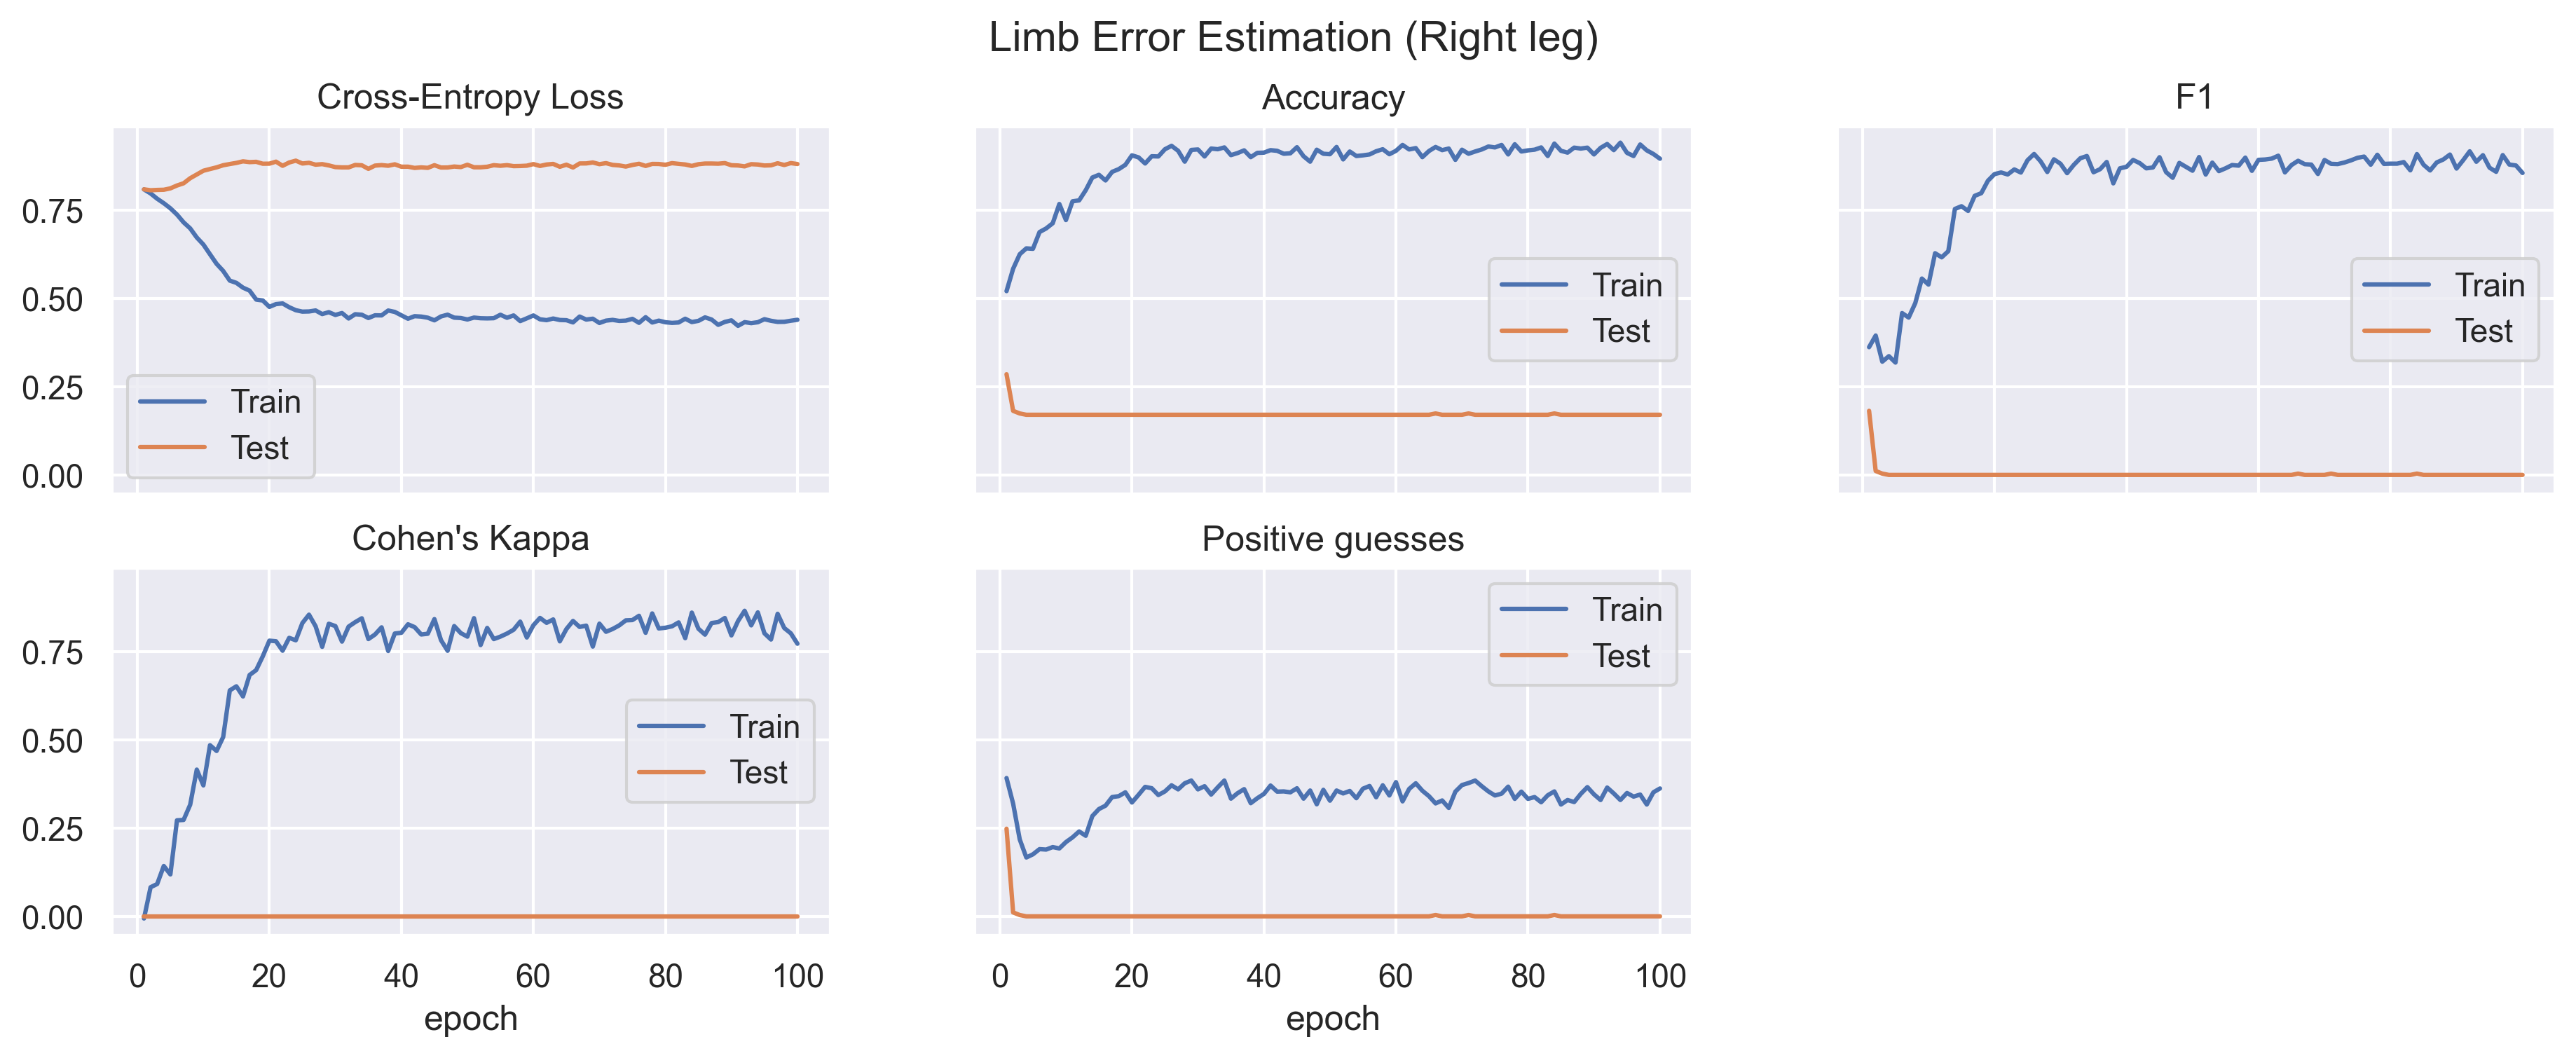
\includegraphics[width=\textwidth]{figures/Results/lb/LimbErrorEstimation_Right leg.png}
      \caption{Right leg Error Estimation}
      \label{fig:rileg_lb_ee}
  \end{subfigure}
  \hfill
  \caption[Limb model training results]{The training results of the limb error estimation model.}
     \label{fig:limb_training_results}
\end{figure}

\subsection{Confusion Matrix}

The confusion matrix of the limb model is shown in Figure \ref{fig:limb_confusion_matrix}. It can be seen that the model only predicts the error label "No Error" or "Error" for most joints without variation. This is because the model is overfitting.

\begin{figure}
  \centering
  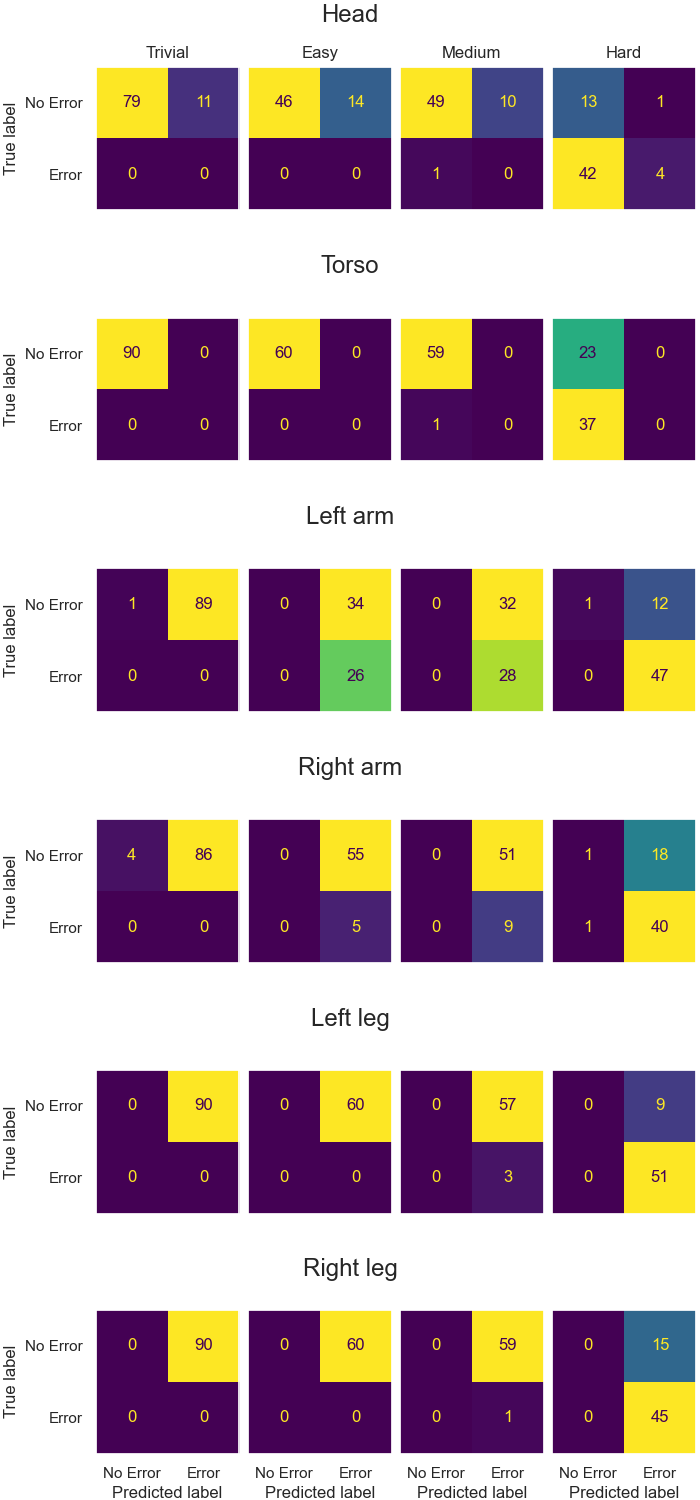
\includegraphics[width=0.8\textwidth]{figures/results/confusion/limbs.png}
  \caption[Limb model confusion matrix]{The confusion matrix of the limb model.}
  \label{fig:limb_confusion_matrix}
\end{figure}

\subsection{Emulated Full Body}

As with the half body Error estimator, the full body is emulated with the result of the limb error estimation. The results can be seen in Figure \ref{fig:limbs_emulated_full_body}. 

\begin{figure}
    \centering
    %\includegraphics[width=0.8\textwidth]{figures/results/Half_Body/Emulated_Full_Body.png}
    \caption[Limb model with emulated Full Body results]{The results of the Limb model when emulating the full body results.}
    \label{fig:limbs_emulated_full_body}
\end{figure}
  
\subsection{Emulated Half Body}

Additionally, the half body is emulated with the result of the limb error estimation. The Head, Torso, and Left and Right arm are considered as the upper body, and the Left and Right leg are considered as the lower body. The results of the model are shown in Figure \ref{fig:limb_emulated_half_body}.

\begin{figure}
    \centering
    %\includegraphics[width=0.8\textwidth]{figures/results/Half_Body/Emulated_Full_Body.png}
    \caption[Limb model with emulated Half Body results]{The results of the Limb model when emulating the half body results.}
    \label{fig:limbs_emulated_half_body}
\end{figure}
